\documentclass[11pt]{article}
\usepackage[utf8]{inputenc}
\usepackage[margin=1in]{geometry}
\usepackage{graphicx}
\usepackage{listings}
\usepackage{xcolor}
\usepackage{hyperref}
\usepackage{float}

\definecolor{codegreen}{rgb}{0,0.6,0}
\definecolor{codegray}{rgb}{0.5,0.5,0.5}
\definecolor{codepurple}{rgb}{0.58,0,0.82}
\definecolor{backcolour}{rgb}{0.95,0.95,0.92}

\lstdefinestyle{mystyle}{
    backgroundcolor=\color{backcolour},   
    commentstyle=\color{codegreen},
    keywordstyle=\color{magenta},
    numberstyle=\tiny\color{codegray},
    stringstyle=\color{codepurple},
    basicstyle=\ttfamily\footnotesize,
    breakatwhitespace=false,         
    breaklines=true,                 
    captionpos=b,                    
    keepspaces=true,                 
    numbers=left,                    
    numbersep=5pt,                  
    showspaces=false,                
    showstringspaces=false,
    showtabs=false,                  
    tabsize=2
}

\lstset{style=mystyle}

\title{Homework \#3 - Simple DL Workflow in GKE \\ \large COMS 6998: Applied Machine Learning in the Cloud}
\author{Dakshinamoorthy A (da3232) \\ Columbia University}
\date{May 8, 2026}

\begin{document}

\maketitle

\section{Objective}
The objective of this assignment is to develop Container and Kubernetes artifacts to perform Deep Learning (DL) training and DL inference hosting in Google Kubernetes Engine (GKE). This involves creating Dockerfiles, Kubernetes manifests (Jobs, Deployments, Services), and managing persistent storage (PVC) to handle model state across different phases of the lifecycle.

\section{Architecture Aspects \& Requirements}
The project implements a simple yet representative DL workload: **MNIST Digit Classification** using PyTorch. The architecture consists of two primary phases:

\subsection{Training Phase}
The training phase is implemented using a \textbf{Kubernetes Job}. 
\begin{itemize}
    \item \textbf{Why Job?}: Training is a finite task with a clear start and end. The Job controller ensures the pod runs until the script completes and the model is saved.
    \item \textbf{Hardware}: The Job requests 1 NVIDIA Tesla T4 GPU to accelerate the training process.
\end{itemize}

\subsection{Inference Phase}
The inference phase is implemented using a \textbf{Kubernetes Deployment} and a \textbf{LoadBalancer Service}.
\begin{itemize}
    \item \textbf{Why Deployment?}: Inference requires high availability and scaling capabilities. The Deployment controller ensures the web server is always running.
    \item \textbf{Interactive UI}: A Flask-based web server provides a canvas for users to draw digits and receive real-time predictions.
\end{itemize}

\section{Implementation Details}

\subsection{Infrastructure Provisioning}
The cluster was created as a Private GKE Cluster in the \texttt{asia-east1-c} zone to comply with project-level security constraints regarding external IP addresses.

\begin{figure}[H]
    \centering
    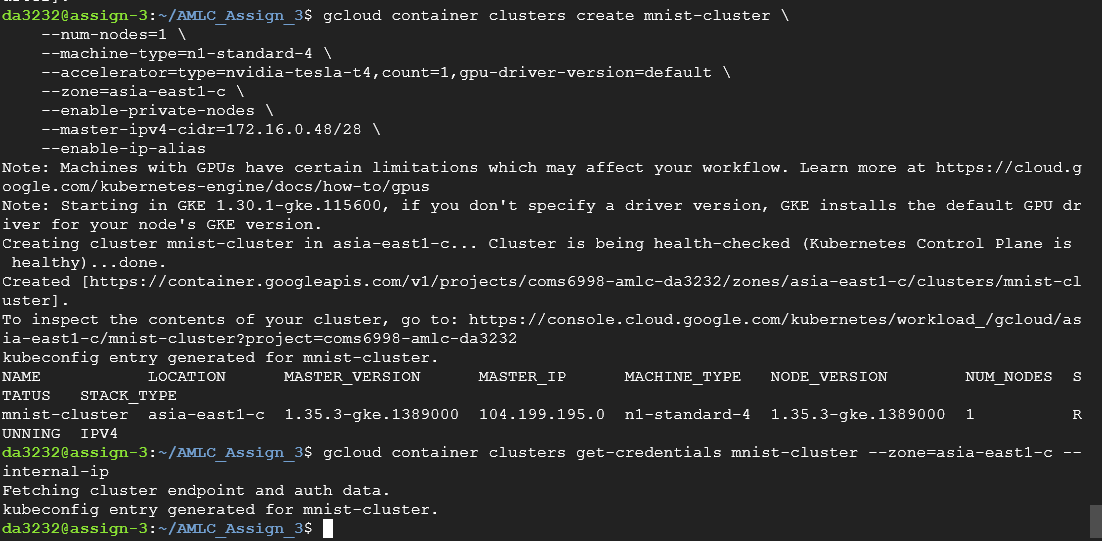
\includegraphics[width=0.8\textwidth]{Screenshots/Cluster Creation.png}
    \caption{GKE Cluster Creation in asia-east1-c}
\end{figure}

\begin{figure}[H]
    \centering
    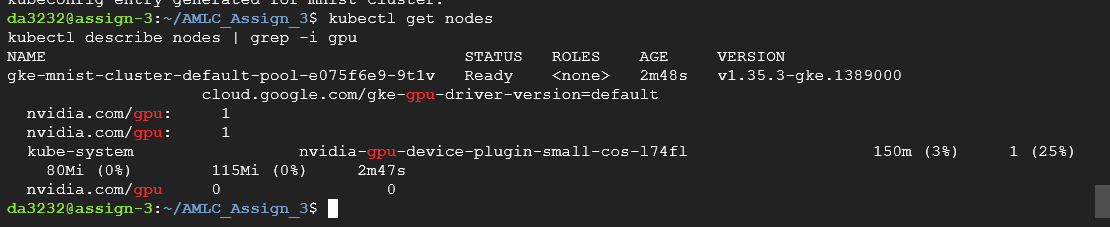
\includegraphics[width=0.8\textwidth]{Screenshots/Kubectl Nodes.png}
    \caption{Verification of Nodes and GPU Availability}
\end{figure}

\subsection{Containerization}
Two separate Dockerfiles were created for training and inference. The images were built and pushed to the Google Artifact Registry.

\begin{figure}[H]
    \centering
    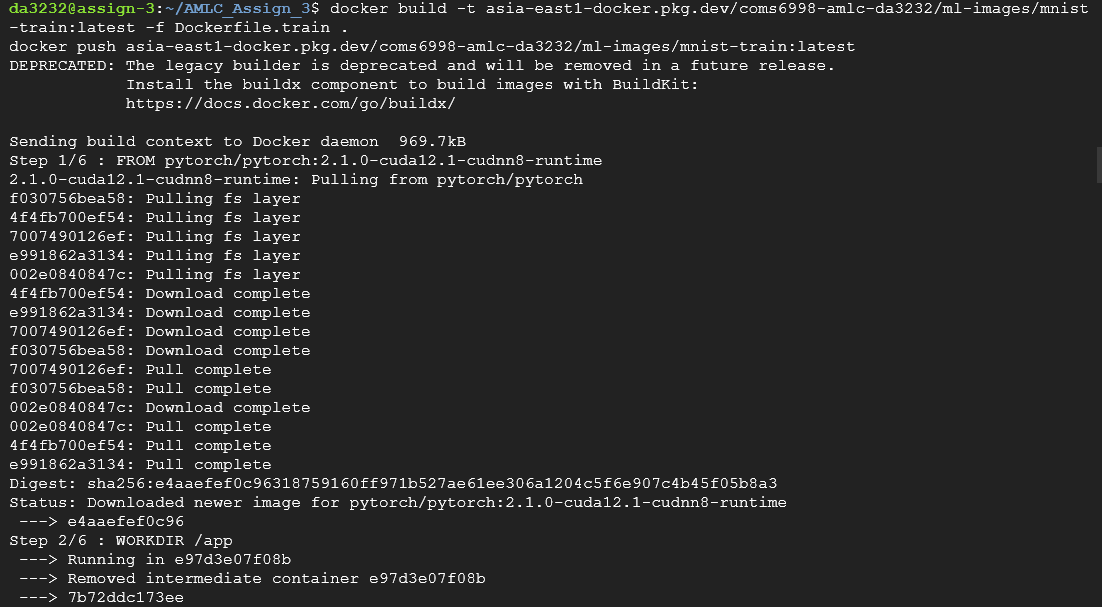
\includegraphics[width=0.7\textwidth]{Screenshots/Docker Build 1.png}
    \caption{Building and Pushing Docker Images (Part 1)}
\end{figure}

\begin{figure}[H]
    \centering
    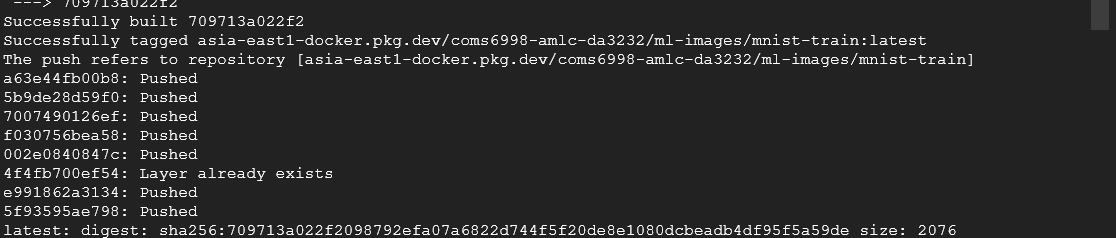
\includegraphics[width=0.7\textwidth]{Screenshots/Docker Build 2.png}
    \caption{Building and Pushing Docker Images (Part 2)}
\end{figure}

\subsection{Persistent Storage (PVC)}
A Persistent Volume Claim was created to store the trained model. This allows the inference pod to load the model saved by the training pod.

\begin{figure}[H]
    \centering
    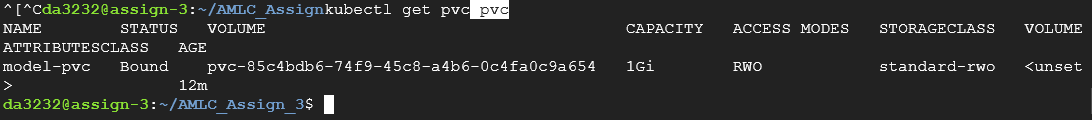
\includegraphics[width=0.8\textwidth]{Screenshots/Get PVC.png}
    \caption{Verification of Bound Persistent Volume Claim}
\end{figure}

\section{Execution and Results}

\subsection{DL Training}
The training job was executed using the GPU. The logs show the model successfully iterating through epochs and saving the result to the PVC.

\begin{figure}[H]
    \centering
    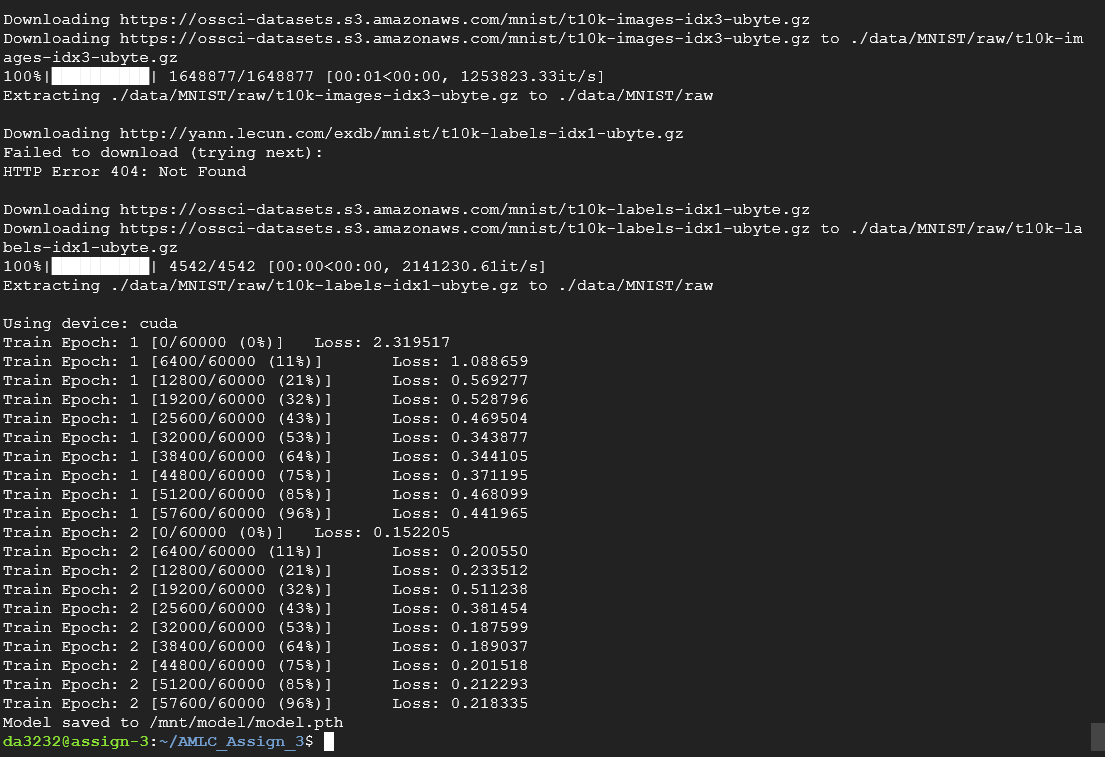
\includegraphics[width=0.8\textwidth]{Screenshots/Training 2.png}
    \caption{Training Logs showing CUDA usage and Model Saving}
\end{figure}

\subsection{Interactive Inference}
The inference engine was exposed via a LoadBalancer. The following screenshots demonstrate the service creation and the interactive UI predicting a hand-drawn digit.

\begin{figure}[H]
    \centering
    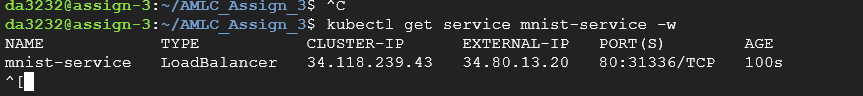
\includegraphics[width=0.8\textwidth]{Screenshots/Inference 1.png}
    \caption{Service Creation and External IP Assignment}
\end{figure}

\begin{figure}[H]
    \centering
    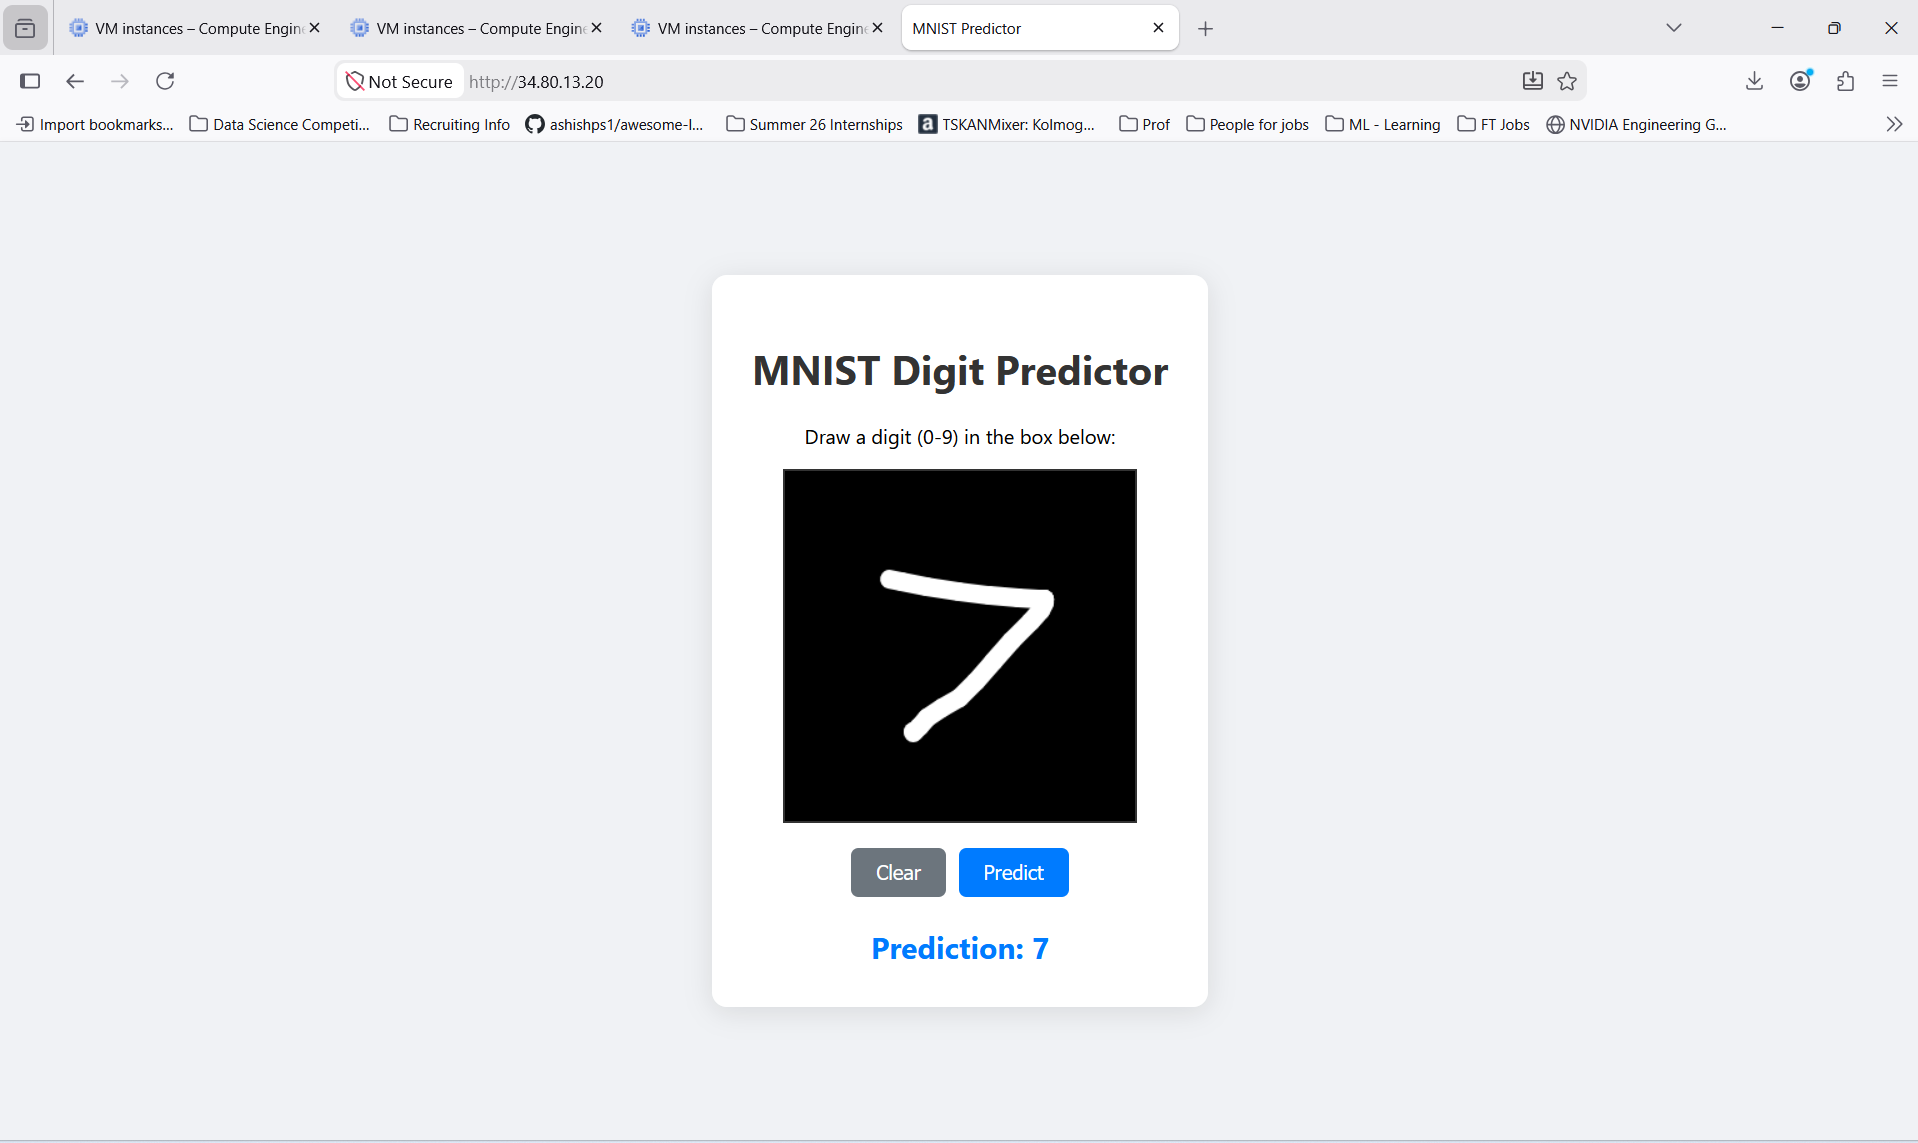
\includegraphics[width=0.9\textwidth]{Screenshots/Inference 2.png}
    \caption{Interactive MNIST Predictor UI}
\end{figure}

\begin{figure}[H]
    \centering
    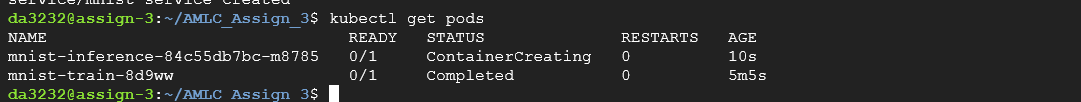
\includegraphics[width=0.8\textwidth]{Screenshots/Kube Pods.png}
    \caption{Status of Kubernetes Pods after Deployment}
\end{figure}

\section{Experience and Reflection}
The primary challenge in this assignment was navigating the specific regional resource availability (GCE Stockouts for GPUs) and security constraints (External IP violations). Implementing a Private GKE Cluster provided a secure and robust solution. The use of native Kubernetes objects (Jobs and Deployments) allowed for a clear separation of concerns between the transient training process and the persistent serving process.

\end{document}
